\documentclass[]{report}

% All Dependencies

\usepackage{graphicx}
\usepackage{float}
\usepackage{amsmath}
\usepackage{amsfonts}
\usepackage{wasysym}


% Title Page
\title{MATH 4820 - Homework 4}
\author{Jack Reilly Goldrick}


\begin{document}
\maketitle


\section{Problem 1}

\subsection{Exercise 2.3.3}

\begin{figure}[H]
	\centering
	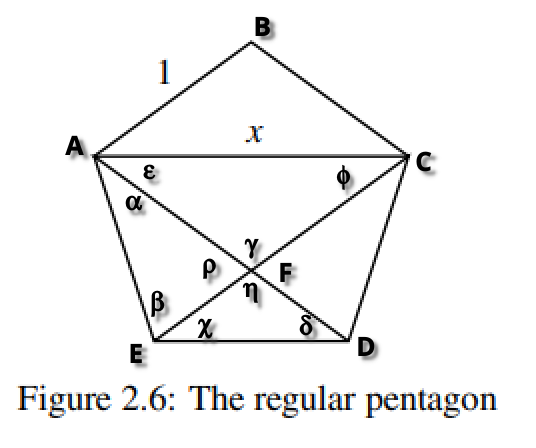
\includegraphics[width=0.7\linewidth]{pics/p1}
\end{figure}


\begin{itemize}

\item We can see that angles $\alpha = \delta = 36^{\circ} $ since $\angle AED = 108^{\circ} $ and $\triangle AED $ is isosceles.  

\subitem Using Opposite interior Angles of Parallel lines we can deduce that $\epsilon = \delta$

\item We can repeat this process for $\triangle EDC$ resulting in $\epsilon = \delta = \chi  = \phi = \alpha  $

\item Thus looking at $\triangle AEC $ we can find $\beta$ by solving the equation for $\beta$:
	
	
	$$ 180 = 3 *x + \beta \  \text{Such that } x = 36^{\circ} $$
	
	\item this results in $\beta = \phi  = 72^{\circ}$ and $\triangle AEF \land \triangle AEC$ being isosceles.  
	
	\item From this we can deduce that segment $EC$ is the same length as $AC$ which is $x$ and that the segment $AF$ has the same length as the sides of the pentagon, 1.
	
	\item thus we have the following relation:
	
	$$ x -1 =  FD$$
	
	\item given the angles and segments making  $\triangle AFD \land \triangle AFC$ similar we can  say:
	$$ \frac{1}{FD} = \frac{x}{1} $$
	
	$$ \frac{1}{x - 1} = \frac{x}{1} $$
	
	\item Thus we have  the desired relation :
	
	
	$$ x = \frac{1}{x - 1} $$
	

\end{itemize}

\begin{flushright}
\smiley{}
\end{flushright}





\section{Problem 2}

\subsection{Exercise 2.3.4}


\begin{figure}[H]
	\centering
	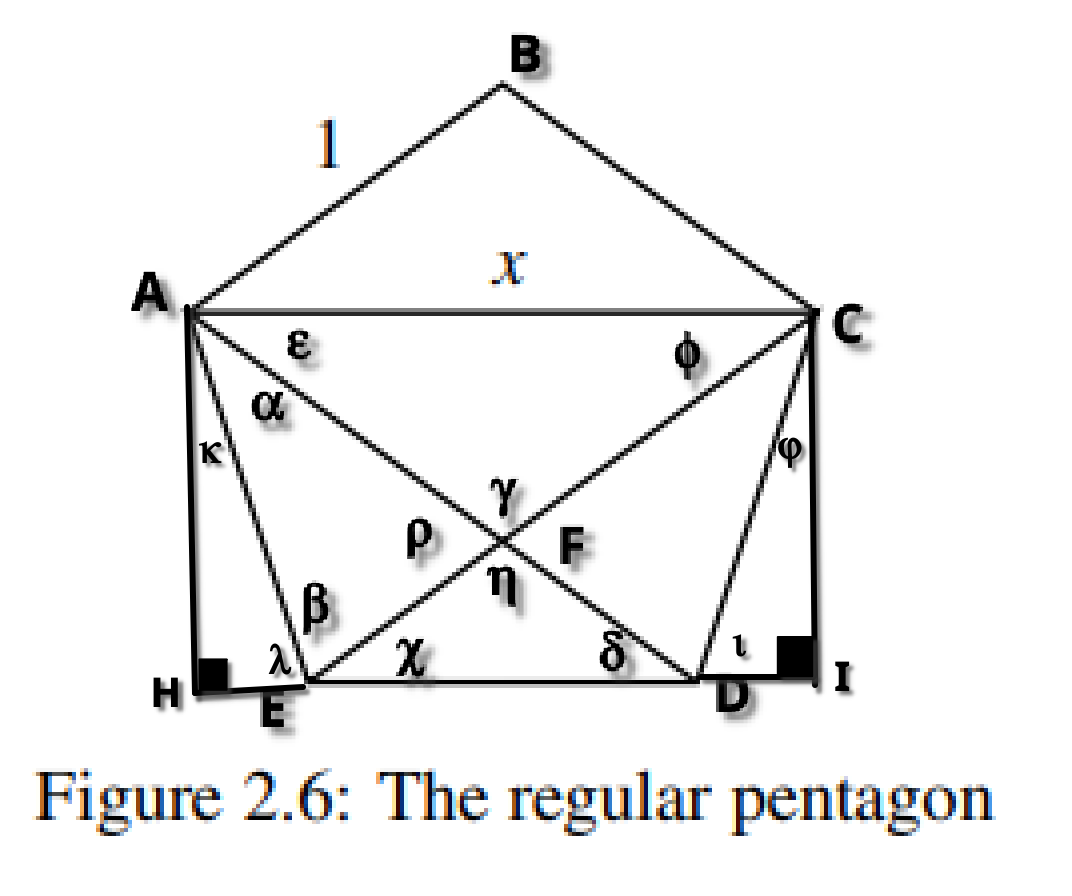
\includegraphics[width=0.7\linewidth]{pics/p2}
\end{figure}

\begin{itemize}
\item The construction can be achieved via creating two new triangles AHE and DCI. Thus we can say:

$$ x  = HE + ED + DI $$

\item We can use the facts of constructible right triangles to show that segments HE and DI are constructible.  

\item Then using the fact that a sum of constructible segments is also cosntructible we can say that the length x is a  result of the sum of three constructible numbers.  

\item Therefore x is constructible.

\end{itemize}

\begin{flushright}
\smiley{}
\end{flushright}



\section{Problem 3}

\begin{figure}[H]
	\centering
	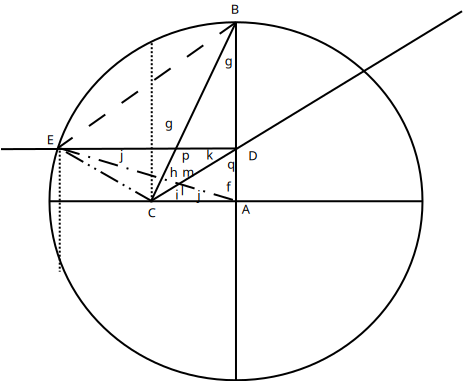
\includegraphics[width=0.7\linewidth]{pics/p3}
\end{figure}

\begin{itemize}
\item To verify the Constructibility of the Pentagon we will show that $\angle{i}$  divides the circle into 5 equal parts.

\item[1.]  Using the equilateral triangles we can construct the midpoint of $\overline{AR}$  called C.

\item[2.]  Forming $\overline{CB}$ we create a right triangle $ABC$.  

\item[3.] Given that the ratios of side lengths are constructible numbers then  angles $g, (h + i),  \land  (j + f)$ are as well through cosine.

\item[4.] Knowing the sum of constructible numbers must also be a constructible number, we can say that angles $ h, i, j \land f$ are constructible as well.

\item[5.] Given that $\overline{CD}$ is the angle bisector of $\angle (h + i)$ and $i$ is opposite interior of $k$,  we can conclude that $h = i = k$.

\item[6.] Exterior Angles and Triangles can be used to derive the equivalence of $m$ and $l$ 

$$ m = 180 - g - f $$

$$ l = q + f $$ 

\item Making the appropriate substitution using the fact that $k$ and $i$ are complementary we have:

$$ f = \frac{90 + g - i}{2}  $$


\item 90, 2, g and I are all constructicble numbers, the process can be repeated 4 more times to validly complete the regular pentagon


\item Therefore this is a valid construction.



\end{itemize}


\begin{flushright}
\smiley{}
\end{flushright}


\end{document}          
